As reasoned in \autoref{sec:ICS} an online offpolicy method which works with a continuous action and observation space is the chosen method due to its sample efficiency. The actor-critic framework is the commonly used to learn an optimal policy for online and continuous domain problems. The actor learns the optimal policy by Q-value maximisation; maximising the expected cumulative return from taking a given action in a given state. So the actor, \(\zeta(s_t; \theta^Z)\), learns the action for each state to maximise expected return through \autoref{eq:maxQ_AC}, with the mapping of state to action learnt through a neural network acting as a function approximator. The critic estimates the state-action value \(Q(s_t, a_t; \theta^Q)\); the expected reward for taking an action in a given state, this is used by the actor to update its policy. The critic is used instead of raw rewards to train the actor because it reduces the variance of policy gradient updates by providing smoothed action-value estimates.

Meanwhile, the critic learns to minimise TD error \footnote{Defined in \autoref{sec:exploration}.}. For example, \autoref{eq:TD_AC} shows the scenairo for a critic where the TD error between the predicted state-action pair and the critic's target network.

\begin{equation}
    \mathcal{L}_Q(\theta^Q) = \frac{1}{N_{\text{buffer}}} \cdot \sum_{i=1}^{N_{\text{buffer}}}(R^i(s^i_t, a^i_t) + \gamma \cdot Q'(s^i_{t+1}, \zeta'(s^i_{t+1};\theta^{\zeta'});\theta^{Q'}) - Q(s^i_t, a^i_t; \theta^Q))^2
\label{eq:TD_AC}
\end{equation}

\begin{equation}
    \mathcal{L}_\zeta(\theta^\zeta) = - \frac{1}{N_\text{buffer}} \cdot \sum_{i=1}^{N_{\text{buffer}}} Q(s^i_t, \zeta(s^i_t;\theta^\zeta);\theta^Q)
\label{eq:maxQ_AC}
\end{equation}

The following subsections cover 5 of the main continuous online offpolicy reinforcement  learning algorithms found in literature. SAC and Maximum a posteriori Policy Optimisation (MPO) learn a stochastic policy, while Deep Deterministic Policy Gradient (DDPG), Distributed Distributional Deterministic Policy Gradient (D4PG) and TD3 learn a deterministic policy.

\subsubsection{Deep Deterministic Policy Gradient method}
\label{sec:DDPG}

DQNs work with a discrete action space, as such with a continuous control problem the continuous outputs have to be discretised leading to massive a massive action dimension, inhibiting learning. DDPG was presented by \cite{lillicrap2015continuous} to be a solution to this problem through an extension to the Deterministic Policy Gradient (DPG) method (\cite{silver2014deterministic}), allowing for a model-free offpolicy online actor-critic algorithm with neural networks utilised as deep function approximators to learn a policy and state-action value function in continuous domains.

The actor provides deterministic actions with the critic approximating the resulting Q-value. \cite{mnih2015human} utilise target networks and experience replay, like in DQNs, to stabilise training and improve sample efficiency, and OU noise is used for action noise-based exploration like explained in \autoref{sec:exploration}.

To summarise DDPG is an actor-critic framework with extensions being:
\begin{enumerate}
    \item Action-space-based noise used for exploration.
    \item Target networks used to improve learning stability, through Polyak averaging \autoref{eq:target_networks}.
\begin{equation}
\begin{aligned}
    \theta^{Q'} \leftarrow& \tilde{\tau} \cdot \theta^Q + (1 - \tilde{\tau}) \cdot \theta^{Q'}\\
    \theta^{\zeta'} \leftarrow& \tilde{\tau} \cdot \theta^\zeta + (1 - \tilde{\tau}) \cdot \theta^{\zeta'}
\end{aligned}
\label{eq:target_networks}
\end{equation}
    \item A replay buffer \(\mathcal{R}\) for off-policy learning, improving sample efficiency.
\end{enumerate}

\begin{tcolorbox}[title={\textbf{Lemma. Target network updates via Polyak averaging}}]
In deep reinforcement learning tasks target networks are often used to stabilise learning by slowly the changing of targets used for value estimation. Instead of directly copying the online netwrok's weights, they are soft updated through \textit{Polyak averaging}..

employed to stabilise learning by providing slowly changing targets for value estimation. Instead of directly copying the online network's weights to the target network, a soft update method called \textit{Polyak averaging} is used.

Let \( \theta \) denote the parameters of the online network and \( \theta^{'}\) the parameters of the corresponding target network. The Polyak update rule is defined as:
\[
    \theta^{'} \leftarrow \tau \theta + (1 - \tau) \theta^{'} 
\]
where \( \tau \in (0, 1) \) is the averaging coefficient, a larger coefficient tracks the target network faster and can induce instability. Alternatively, a small coefficient gives stable but slower updates which can enhance robustness.

Polyak averaging ensures the parameters of the target network move slowly towards that of the online network, reducing oscillations and divergence in value estimation, to promote learning stability.
\end{tcolorbox}

\subsubsection{Distributed Distributional Deterministic Policy Gradients}
\label{sec:D4PG}

\cite{barthmaron2018d4pg} extended DDPG to D4PG to include a distributional critic promotes learning stability, along with PER for faster learning and N-step returns for improving the rewards over longer-time horizons.
\begin{itemize}
    \item A distributed framework is used, where multiple actors asynchronously generate experiences and fill a shared replay buffer, where a central learner updates the policy.
    \item A \textit{distributional critic} is used, essentially instead of modelling a scalar \(Q(s,a; \theta^Q)\) it predicts a probability distribution \(Q_Z(s,a; \theta^{Q_Z})\) over all possible returns, this distribution modelling works well for stochastic environments where differing Q values can come from different actions in the same state. The critic now outputs a probability distribution leading to KL divergence used instead of MSE for the loss function.
    \item N-steps are used to give the reward over a longer time horizon, this is beneficial for task where there are long-term dependencies, such as in rocket landing. The N-step reward equation is shown in \autoref{eq:N_step_rewards}.
\end{itemize}

\begin{equation}
    y^i_t = \bigg(\sum_{m=0}^{N_{\text{episode}}} \gamma^m \cdot R(a^i_m, s^i_m)\bigg) + \gamma^{N_{\text{episode}}} \cdot Q_Z'(s^i_{N_{\text{episode}}}, \zeta'(s^i_{N_{\text{episode}}}; \theta^{\zeta'}); \theta^{Q'})
\label{eq:N_step_rewards}
\end{equation}

\begin{tcolorbox}[title={\textbf{Lemma. N-step returns}}]
In traditional TD learning the value estimate of a state is updated based on the immediate reward and the estimated discounted value of the next state. \autoref{eq:one_step_rewards} is the equation for calculated the 1-step return at time t ($G_t^{(1)}$ ) using the immediate reward ($R_{t+1}$) and the estimated value of the next state ($V(s_{t+1})$).

% $G_t^{(1)}$ is the 1-step return at time t
% $R_{t+1}$ is the immediate reward
% $\gamma$ is the discount factor
% $V(S_{t+1})$ is the estimated value of the next state

\begin{equation}
    G_t^{(1)} = R_{t+1} + \gamma V(s_{t+1})
\label{eq:one_step_rewards}
\end{equation}

N-step returns extends this concept to look ahead $n$ steps through \textit{booststrapping} the fine value estimate.ping. \autoref{eq:n_step_rewards} shows the generic formula for n-step rewards. N-step returns allows the agent to learn from a longer sequence of rewards before bootstrapping, giving it more information about long-term dependencies

\begin{equation}
    G_t^{(n)} = R_{t+1} + \gamma R_{t+2} + \gamma^2 R_{t+3} + ... + \gamma^{n-1} R_{t+n} + \gamma^n V(S_{t+n})
\label{eq:n_step_rewards}
\end{equation}

This formula changes when terminal states are within the trajectory length set for n-step returns ($n$), otherwise called within the n-step horizon. The returns should only include rewards up to the terminal state, either a truncated or completed episode, with no bootstrapping or rewards after termination. If step $t+k$ is a terminal state,where $k < n$), the n-step return becomes \autoref{eq:n_step_rewards_terminal}.

\begin{equation}
    G_t^{(n)} = R_{t+1} + \gamma R_{t+2} + ... + \gamma^{k-1} R_{t+k}
\label{eq:n_step_rewards_terminal}
\end{equation}
\end{tcolorbox}

\subsubsection{Twin Delayed DDPG}
\label{sec:TD3}


\cite{fujimoto2018addressing} use double Q-learning in an actor-critic format to reduce overestimation bias of the value function through a pair of independent critics and double Q-learning. Through their approach, they run DDPG with two extensions:
\begin{enumerate}
    \item Clipped Gaussian noise is used instead of OU for action space-based noise; clipped noise is chosen to prevent sharp action value changes causing over-fitting.
    \item Through the use of double Q-learning (dual critics), the loss functions for the critic have the "target critic changed" to the minimum between the networks, ensuring the most conservative estimate. For the actor loss, only the primary Q-network is considered; this ensures it is based on a single Q-value estimate reducing noise and learning instability.
\end{enumerate}

\subsubsection{Soft Actor-Critic}
\label{sec:SAC}

\cite{haarnoja2018soft} introduce SAC as an actor-critic algorithm which maximises both expected rewards and the policy's entropy, encouraging exploration and thus leading to more robust policies. 
TD3 uses Gaussian action space noise, whereas SAC's actor outputs a Gaussian distribution \(\zeta_S(s;\theta^{\tilde{\zeta}}, \theta^\mu, \theta^\sigma)\), with the subscript "S" denoting it as a stochastic actor. This actor outputs \(\mu(s_t; \theta^\mu)\) and \(\sigma(s_t; \theta^\mu)\), which are converted to a noisy action through \autoref{eq:SAC_actor}. Compared to TD3, the difference is that the noise distribution is a learned parameter providing \textit{state-dependent exploration}.

\begin{equation}
\begin{aligned}
    \sigma(s; \theta^\mu) = e^{\log \sigma(s; \theta^\mu)} ,\quad
    \tilde{a} = \mu(s; \theta^\mu) + \sigma(s; \theta^\mu) \odot \epsilon ,\quad
    \epsilon \sim \mathcal{N}(0,I) ,\quad
    a = tanh(\tilde{a})
\end{aligned}
\label{eq:SAC_actor}
\end{equation}

\begin{figure}[H]
    \centering
    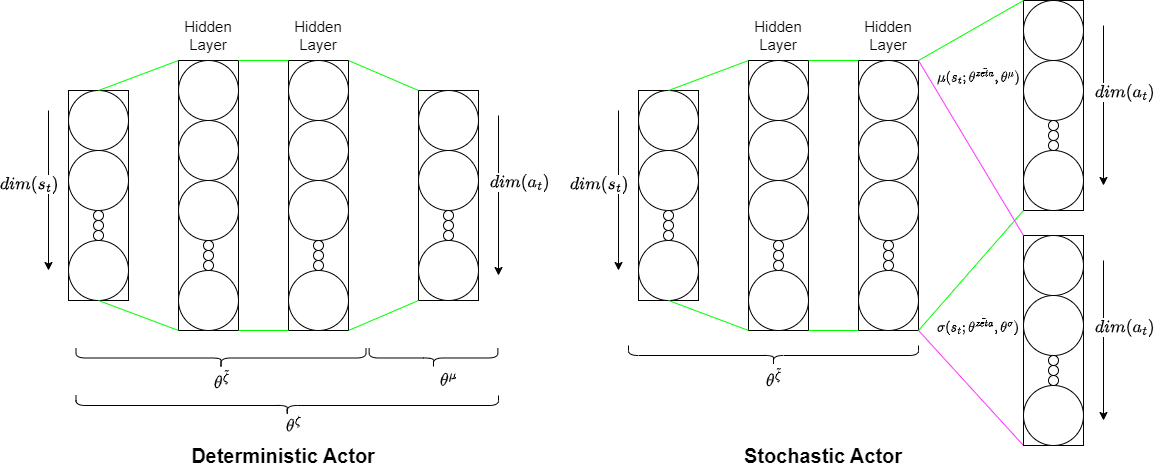
\includegraphics[width=0.95\linewidth]{figures/LiteratureStudy/RL_diagram_ActorNetworks.png}
    \caption{Diagram showing the differences in actor networks, for deterministic and stochastic.}
    \label{fig:actor_networks}
\end{figure}

SAC has an additional entropy term to control the state-dependent exploration. \textit{Temperature} $v$ updates to encourage an entropy to meet the target entropy controlling the degree of randomness and traditionally set as  \(\mathcal{H}_{\text{target}} := -\dim(a_t)\). \autoref{eq:SAC_temperature} temperature is updated to encourage the negative Gaussian likelihood equal to the target entropy.

\begin{equation}
    \mathcal{L}_{\log(\nu)} = \frac{1}{N} \cdot \sum_{i=1}^{N}-\log(\nu) \cdot \bigg(\log p(a_t^i|\mu,\sigma^2)+\mathcal{H}_{\text{target}}\bigg)
\label{eq:SAC_temperature}
\end{equation}


\begin{tcolorbox}[title={\textbf{Lemma. Gaussian likelihood}}]
The Gaussian likelihood is the probability density function of a normal distribution evaluated at a given point. For a random variable \( x \in \mathbb{R}^d \), with mean \( \mu \in \mathbb{R}^d \) and standard deviation \( \sigma \in \mathbb{R}^d \), the log-likelihood is given by:
\[
\log p(x \mid \mu, \sigma^2) = -\frac{1}{2} \left[ \frac{(x - \mu)^2}{\sigma^2} + 2 \log \sigma + \log(2\pi) \right]
\]
The Gaussian likelihood shows how likely point $x$ is under the $\mu$ and $\sigma^2$. The first term is called the \textit{quadratic term} and penalises deviations from the mean scaled by the variance. The second term called the \textit{normalisation term} accounts for the distribution spread, and the final term is a constant ensuring proper normalisation.

A lower negative log probability, \textit{Gaussian likelihood}, indicates the sample is more likely under the distribution, while a high negative log probability indicates a less likely sample under the distribution.
\end{tcolorbox}

The actor has two terms in its loss function, first an entropy regularisation term, where the log probability gives a metric for the likelihood of the actor, weighted by the temperature. The temperature updates previously to balance entropy through changing the entropy regularisation loss magnitude in the reward function. The second term extracts the minimum of two q network outputs, alike double q-learning, to reduce overestimation bias; this term encourages the policy to select the actions of that state with the highest expected returns.

\begin{equation}
    \mathcal{L}_{\zeta^S} = \frac{1}{N} \cdot \sum^N_{i=1} \bigg(\nu \cdot \log p(a_t^i|\mu, \sigma^2) - \min_{i=1,2}Q(s_t^i,a_t^i;\theta^{Q_i})\bigg)
\label{eq:SAC_actorloss}
\end{equation}

The TD error is computed to represent the mean-squared Bellman error for each critic, which is trained to minimised the square difference between its predicted Q-value and the shared TD target, through the loss function of \autoref{eq:SAC_critic_loss}.

\begin{equation}
\begin{aligned}
    TD_{\text{target}} =& R_t + \gamma \cdot (1-d) \cdot \bigg(\min_{i=1,2} \{Q'(s',a';\theta^{Q'})\}- \nu \cdot \log p(a'|\mu',(\sigma')^2)\bigg) \\
    e_{TD} =& \frac{1}{2} \cdot \bigg((TD_{\text{target}} - Q_1)^2 + (TD_{\text{target}} - Q_2)^2\bigg)
\end{aligned}
\label{eq:TD_error_entropy_regularised}
\end{equation}

\begin{equation}
    \mathcal{L}_Q = \frac{1}{N} \cdot \sum^N e_{TD}
\label{eq:SAC_critic_loss}
\end{equation}

% SAC in a distributed format
SAC has been used to perform many tasks, \cite{wahid2020learning} used it in a distributed form to perform control and navigation tasks. While \cite{akimov2019distributed} used it in a distributed framework to update a shared replay buffer and used a multivariate reward representation to have sub-rewards allowing for transfer learning, which utilises knowledge distillation to increase learning speed.

% STOPPED HERE
\subsubsection{Maximum a posteriori Policy Optimisation}
\label{sec:MPO}

\cite{schulman2015trpo} introduced Trust Region Policy Optimisation (TRPO) as an iterative procedure for policy optimisation suitable to large non-linear policies of neural networks. Here a trust region controls the update between policies through Kullback-Leibler (KL) divergence. \cite{schulman2017proximal} presented Proximal Policy Optimisation (PPO) as a first-order approximation of the second-order optimisation TRPO. The paper states have PPO is simler, more generic and of better sample efficiency than TRPO, and consistently outperforms other onpolicy online methods like Advantage Actor-Critic (A2C).

PPO is a stochastic actor-critic framework which prevents large updates causing instability through constraints on the deviation of the policy through their KL divergence.

\begin{tcolorbox}[title={\textbf{Lemma. KL divergence}}]
The KL divergence is a measure of how one probability distribution \( P \) diverges from a second, reference distribution \( Q \). For continuous distributions with probability densities \( p(x) \) and \( q(x) \), the KL divergence from \( Q \) to \( P \) is defined as:
\[
\mathcal{D}_{\mathrm{KL}}(P \parallel Q) = \int p(x) \log \frac{p(x)}{q(x)} \, dx
\]
The smaller the KL divergence the more identical the distributions are.
\end{tcolorbox}

PPO was first employed without a value function, where the advantage estimate \(\hat{A}_t\) is equal to the Monte Carlo return \(G_t(s_t, a_t) = \sum_{k=0}^\infty \gamma^k \cdot R_{t+k}(s_t, a_t) \). From here, a clipped surrogate objective is used to update the policy, as shown through the second equation in \autoref{eq:PPO}. Note that the other objectives, including a KL divergence-based penalty, were used and showed decreased performance.

\begin{equation}
\begin{aligned}
    \text{No clipping or penalty:}& \mathcal{L}(\theta) = r_t(\theta) \cdot \hat{A}_t(s_t, a_t) \\
    \text{Clipped:}& \mathcal{L}(\theta) = \min\{r_t(\theta)\cdot\hat{A}_t(s_t, a_t), \text{clip}(r_t(\theta), 1 - \epsilon^{\text{PPO}}, 1 + \epsilon^{\text{PPO}}) \cdot \hat{A}_t(s_t, a_t) \\
    \text{KL penalty:}& \mathcal{L}(\theta) = r_t(\theta) \cdot \hat{A}_t(s_t, a_t) - \beta^{\text{PPO}} \cdot \text{KL}[\zeta_{\text{old}}(s_t; \theta^{\zeta_{\text{old}}}) || \zeta(s_t; \theta^\zeta)] \\
    \text{With:}& r_t(\theta) = \frac{\zeta(s_t; \theta^\zeta)}{\zeta_{\text{old}}(s_t; \theta^{\zeta_{\text{old}}})}
\end{aligned}
\label{eq:PPO}
\end{equation}

The actor-critic PPO was introduced to improve sample efficiency via value function estimation to stabilise the advantage function estimate by \autoref{eq:PPO_critic}. Here, the critic is trained to minimise the value loss through MSE \(MSE[G_t, V_t]\).

\begin{equation}
\begin{aligned}
    G_t(s_t, a_t) =& \sum_{k=0}^\infty \gamma^k \cdot R_{t+k}(s_t, a_t) \\
    A_t(s_t, a_t) =& G_t(s_t, a_t) - V(s_t; \theta^\zeta) \\
\end{aligned}
\label{eq:PPO_critic}
\end{equation}

%MPO
\cite{abdolmaleki2018maximum} introduce MPO as an off-policy version to PPO, which has better sample efficiency. They state it boasts the robustness, insensitivity to hyperparameter changes, and scalability of an on-policy algorithm while having the off-policy sample efficiency due to their utilisation of a replay buffer. MPO decouples PPO into two steps:
\begin{enumerate}
    \item Optimisation of a non-parametric target policy.
    \begin{itemize}
        \item The intermediate policy with a probabilistic representation of the value function.
        \item \(\nu\) controls the steepness of distribution, in essence controlling the exploration-exploitation trade-off.
        \item It doesn't rely on a neural network and is computed for the value function, acting like a "soft target" or a reference policy.
    \end{itemize}
    \item Parametric policy updating for target approximation.
    \begin{itemize}
        \item The actual policy which the agent uses to interact with the environment, parametrised through a neural network.
        \item Updates through minimisation of the KL divergence with its non-parametric policy.
    \end{itemize}
\end{enumerate}

The target policy is updated through \autoref{eq:Estep} called the \textit{E-Step} (expectation step). Note that the actor is stochastic, like SAC.

\begin{equation}
    \zeta_{\text{S, target}}(s_t; \theta^{\zeta_{\text{target}}}) \varpropto  \exp\left(\frac{Q(s, a)}{\nu}\right)
\label{eq:Estep}
\end{equation}

The parametric policy is updated through minimisation of the KL divergence of the target and parametric network, as shown in \autoref{eq:PPO}, incorporating  KL divergence constraint to stay within the trust region. Meanwhile, the critic is updated as normal.

The temperature parameter is updated through dual optimisation of \autoref{eq:MPO_dual}, here \(\epsilon^\nu\) controls the variance of the weights for regularisation. \cite{prior2024jaxrl}, use Sequential Least Squares Programming (SLSQP) is used to minimise the dual function concerning $\nu$, with a softmax function used to normalise the new weights, \autoref{eq:MPO_softmax}.


\begin{equation}
    g(\eta) = \nu \cdot \epsilon^{\nu} + \eta \cdot [\mathbb{E}_{s\sim R}[\log(\frac{1}{N_{\text{buffer}}}\cdot\sum_{i=1}^{N_{\text{buffer}}}\exp(\frac{Q(s, a_i; \theta^Q)}{\nu^*}))]]
\label{eq:MPO_dual}
\end{equation}

\begin{equation}
    w_i = \frac{\exp(\frac{Q(s, a_i)}{\eta})}{\sum_j \exp(\frac{Q(s, a_j)}{\eta})}
\label{eq:MPO_softmax}
\end{equation}

The actor updates through the log-likelihood of the target and current policies, as is a multi-variate Gaussian distribution. Secondly, it has two Lagrangian multipliers \(\lambda^\mu\) and \(\lambda^\sigma\) to maintain the constraints on the KL divergence between the target and current policy's Gaussian distributions. Pre-defined thresholds \(M^\mu\) and \(M^\sigma\) define the \textit{trust region}. This process is shown in \autoref{eq:MPO_actor}.

\begin{equation}
\begin{aligned}
    \mathcal{L}^\sigma &= \lambda^\sigma \cdot \left(M^\sigma - D_{KL}(\zeta^{\text{target}}(s_t; \theta^\sigma) \parallel \zeta(s_t; \theta^\sigma))\right), \\
    \mathcal{L}^\mu &= \lambda^\mu \cdot \left(M^\mu - D_{KL}(\zeta^{\text{target}}(s_t; \theta^\mu) \parallel \zeta(s_t; \theta^\mu))\right), \\
    \mathcal{L}^{\zeta, \text{unconstrained}} &= - \frac{1}{N^{\text{buffer}}} \sum_{i=1}^{N^{\text{buffer}}} \Big( \log P(a_i \mid \mu^{\text{target}}(s_t; \theta^\mu), \sigma(s_t; \theta^\sigma)) \\
    &\quad + \log P(a_i \mid \mu(s_t; \theta^\mu), \sigma^{\text{target}}(s_t; \theta^{\sigma^{\text{target}}})) \Big).
\end{aligned}
\label{eq:MPO_actor}
\end{equation}


The \textit{"Maximum a Posteriori"} framework balances the exploration-exploitation trade-off through a trust region. Like SAC, a temperature parameter \(\nu\) controls the system's entropy. The authors tested it on control tasks \textit{Walker-2D}, \textit{Acrobat}, and \textit{Hopper}; it was shown to outperform DDPG and PPO in an extensive ablation study. However, there is limited evidence of whether it can outperform more advanced DDPG algorithms like D4PG, SAC or TD3.

\cite{prior2024jaxrl} implement this scheme in JAX (\cite{jax2018github}) with a double critic alike TD3. Deduced to be used to reduce overestimation bias; secondly, they clip the gradient of the loss function for the actor update. Finally, target networks are used.

The original paper runs the MPO algorithm in a distributed form, with a single learner but multiple learners (agents) collecting data independently, with a \text{chief} collecting the gradients and performing a parameter update through averaging gradients. In other words, \textit{distributed synchronous SGD}.


Finally, MPO can be used in a distributed framework, with the user able to configure it however they like. \cite{hoffman2020acme} implemented DMPO in their Acme framework, using distributional critics similar to D4PG.